\documentclass{xjtureport}
% =============================================
% Part 0 Edit the info
% =============================================

\major{计算机001班}
\name{曾锦程}
\title{SDN实验报告}
\stuid{2203613040}
\college{计算机学院}
\date{\zhtoday}
\lab{}
\course{软件定义网络}
\instructor{张鹏}
\grades{}
\expname{Lab2 自学习交换机与广播风暴}
\exptype{设计实验}
\partner{}

\begin{document}
% =============================================
% Part 1 Header
% =============================================
\makecover
\makeheader

% =============================================
% Part 2 Main document
% =============================================

\section{实验任务一:自学习交换机}
\subsection{背景介绍}
\begin{figure}[H]
	\centering
	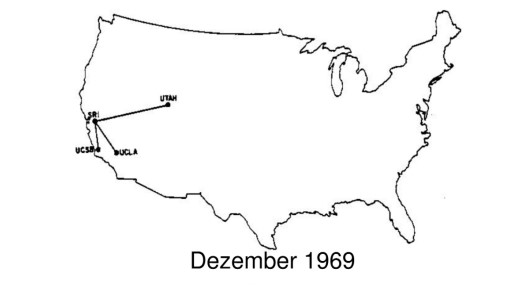
\includegraphics[width=0.8\linewidth]{1.jpg}
	\caption{ARPANET-1}
\end{figure}
1969年的\textbf{\texttt{ARPANET}}非常简单,仅由四个结点组成。假设每个结点都对应一个交换机,每个交换机都具有
一个直连主机,你的任务是实现不同主机之间的正常通信。
前文给出的简单交换机洪泛数据包,虽然能初步实现主机间的通信,但会带来不必要的带宽消耗,并且
会使通信内容泄露给第三者。因此,请你在简单交换机的基础上实现二层自学习交换机,避免数据包的
洪泛。
\subsection{自学习交换机原理}
(a) 控制器为每个交换机维护一个 \textbf{mac-port} 映射表。\par
(b) 控制器收到 \textbf{packet\_in} 消息后,解析其中携带的数据包。\par
(c) 控制器学习 \textbf{src\_mac - in\_port} 映射。\par
(d) 控制器查询 \textbf{dst\_mac} ,如果未学习,则洪泛数据包;如果已学习,则向指定端口转发数据包
( \textbf{packet\_out} ),并向交换机下发流表项( \textbf{flow\_mod} ),指导交换机转发同类型的数据包。
\subsection{关键代码设计思路}
\subsubsection{未考虑Buffer代码}
在构造函数中添加一个全局mac与port映射表,相当于存储所有传统交换机的mac表。
\begin{lstlisting}[language=Python]
	self.mac_to_port = {}
\end{lstlisting}
\quad \quad 将收到的包源mac地址与接收端口对应,相当于传统交换机自学习mac表的过程。
\begin{lstlisting}[language=Python]
	self.mac_to_port[dpid][src] = in_port
\end{lstlisting}
\quad \quad 将收到的包与映射表匹配,如果能匹配到,则输出端口为表中端口,如果匹配不到,则洪泛数据包。
\begin{lstlisting}[language=Python]
	#if match, then send to outport
	if dst in self.mac_to_port[dpid]:
		out_port = self.mac_to_port[dpid][dst]
	#if not match, then flood
	else:
		out_port = ofp.OFPP_FLOOD
\end{lstlisting}
\quad \quad 控制器对交换机作出指示,如果输出端口不是洪泛,添加流表项,增加匹配次数,完成数据包的转发,如果洪泛,则直接转发。
\begin{lstlisting}[language=Python]	
	#pass information
	actions = [parser.OFPActionOutput(out_port)]
	if out_port != ofp.OFPP_FLOOD:
		match = parser.OFPMatch(in_port=in_port, eth_dst=dst, eth_src=src)
		self.add_flow(dp, 1, match, actions)
	data = msg.data	
	out = parser.OFPPacketOut(datapath=dp,buffer_id=msg.buffer_id,in_port=in_port, actions=actions, data=data)
	dp.send_msg(out)	
\end{lstlisting}
\subsubsection{基于Buffer的代码改进}
Buffer是交换机中的概念,意思就是说数据包发入交换机,交换机之后与控制器交互,此时可以不把整个数据包发给控制器,可以通过Bufferid进行通信,以下是对三种消息基于Buffer改进的介绍:\par 
(a)  Packetin消息:用于标记缓存在交换机中的数据报文id,如报文被action上送到控制器中maxlen字段或者table\_miss消息限制长度,而通过bufferid将报文缓存在交换机中,以便被另外两种消息来调用;\par
(b)  Packetout消息:用于控制器将原先buffer在交换机中的报文,通过Packetout个形式从交换机的某个物理口送出去;\par
(c)  Flowmod消息:如果flowmod中带有bufferid,那么说明这个flowmod需要做两件事情,第一是正常下发一条flow,其次是把交换机中先前buffer的那个数据报文,Packetout到table来匹配一次下的这条flow;注意以上两个指令都是通过这个带有bufferid的消息执行的,不需要控制器另外下packet\_out消息,这种设计思路是非常巧妙的。\par  
(d)代码修改:\par
首先将add\_flow函数修改成能够支持Buffer机制的函数,即支持上文介绍的Buffer机制的Flowmod。
\begin{lstlisting}[language=Python]	
def add_flow(self, datapath, priority, match, actions,buffer_id=None,idle_timeout=0,hard_timeout=0):
	dp = datapath 
	ofp = dp.ofproto 
	parser = dp.ofproto_parser 
	inst = [parser.OFPInstructionActions(ofp.OFPIT_APPLY_ACTIONS, actions)] 
	if buffer_id: 
		mod = parser.OFPFlowMod(datapath=datapath, priority=priority,buffer_id=buffer_id,idle_timeout=idle_timeout,
		hard_timeout=hard_timeout,match=match,instructions=inst)
	else:
		mod = parser.OFPFlowMod(datapath=datapath, priority=priority,idle_timeout=idle_timeout,
		hard_timeout=hard_timeout,match=match, instructions=inst)
dp.send_msg(mod) 
\end{lstlisting}
在代码中加入以下逻辑:\par
(1)输出不是洪泛的情况下,如果支持Buffer机制的话,直接发出支持Buffer机制的Flowmod消息即可(此时不需要Packetout,可以直接return,因为原报文重新发到table匹配)。\par
(2)如果是支持Buffer机制且输出洪泛的话,将数据data置为空,Packetout只需要传输一个buffer\_id即可转发消息。\par
\begin{lstlisting}[language=Python]
    actions = [parser.OFPActionOutput(out_port)]
	if out_port != ofp.OFPP_FLOOD:
		match = parser.OFPMatch(in_port=in_port, eth_dst=dst, eth_src=src)
		if msg.buffer_id != ofp.OFP_NO_BUFFER:
			self.add_flow(dp, 1, match, actions, msg.buffer_id)
			return
		else:
			self.add_flow(dp, 1, match, actions)
	data = None
	if msg.buffer_id == ofp.OFP_NO_BUFFER:
		data = msg.data
	out = parser.OFPPacketOut(datapath=dp,buffer_id=msg.buffer_id,in_port=in_port, actions=actions, data=data)
	dp.send_msg(out)
\end{lstlisting}
\subsection{运行结果与分析}
可以由图2,图3看出在UCLA ping UTAH的过程中,数据包不再发给UCSB,实现了自学习交换机。
\begin{figure}[H]
	\centering
	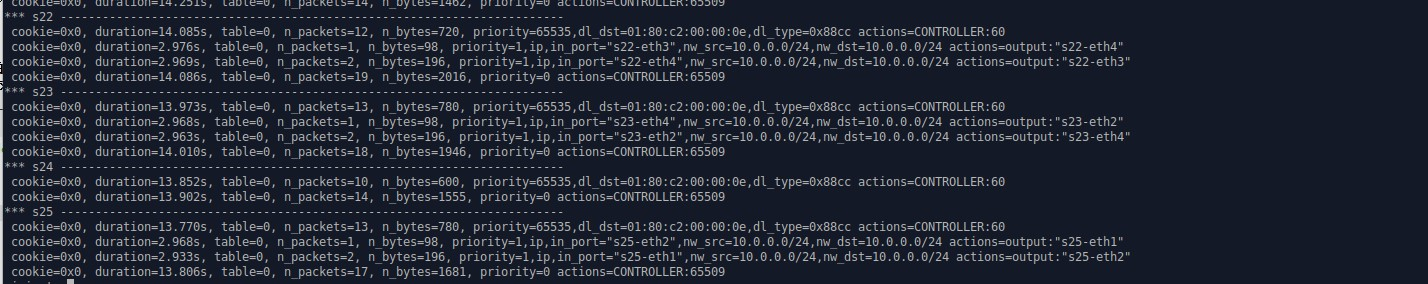
\includegraphics[width=0.8\linewidth]{3.jpg}
	\caption{UCLA  ping  UTAH}
\end{figure}
\begin{figure}[H]
	\centering
	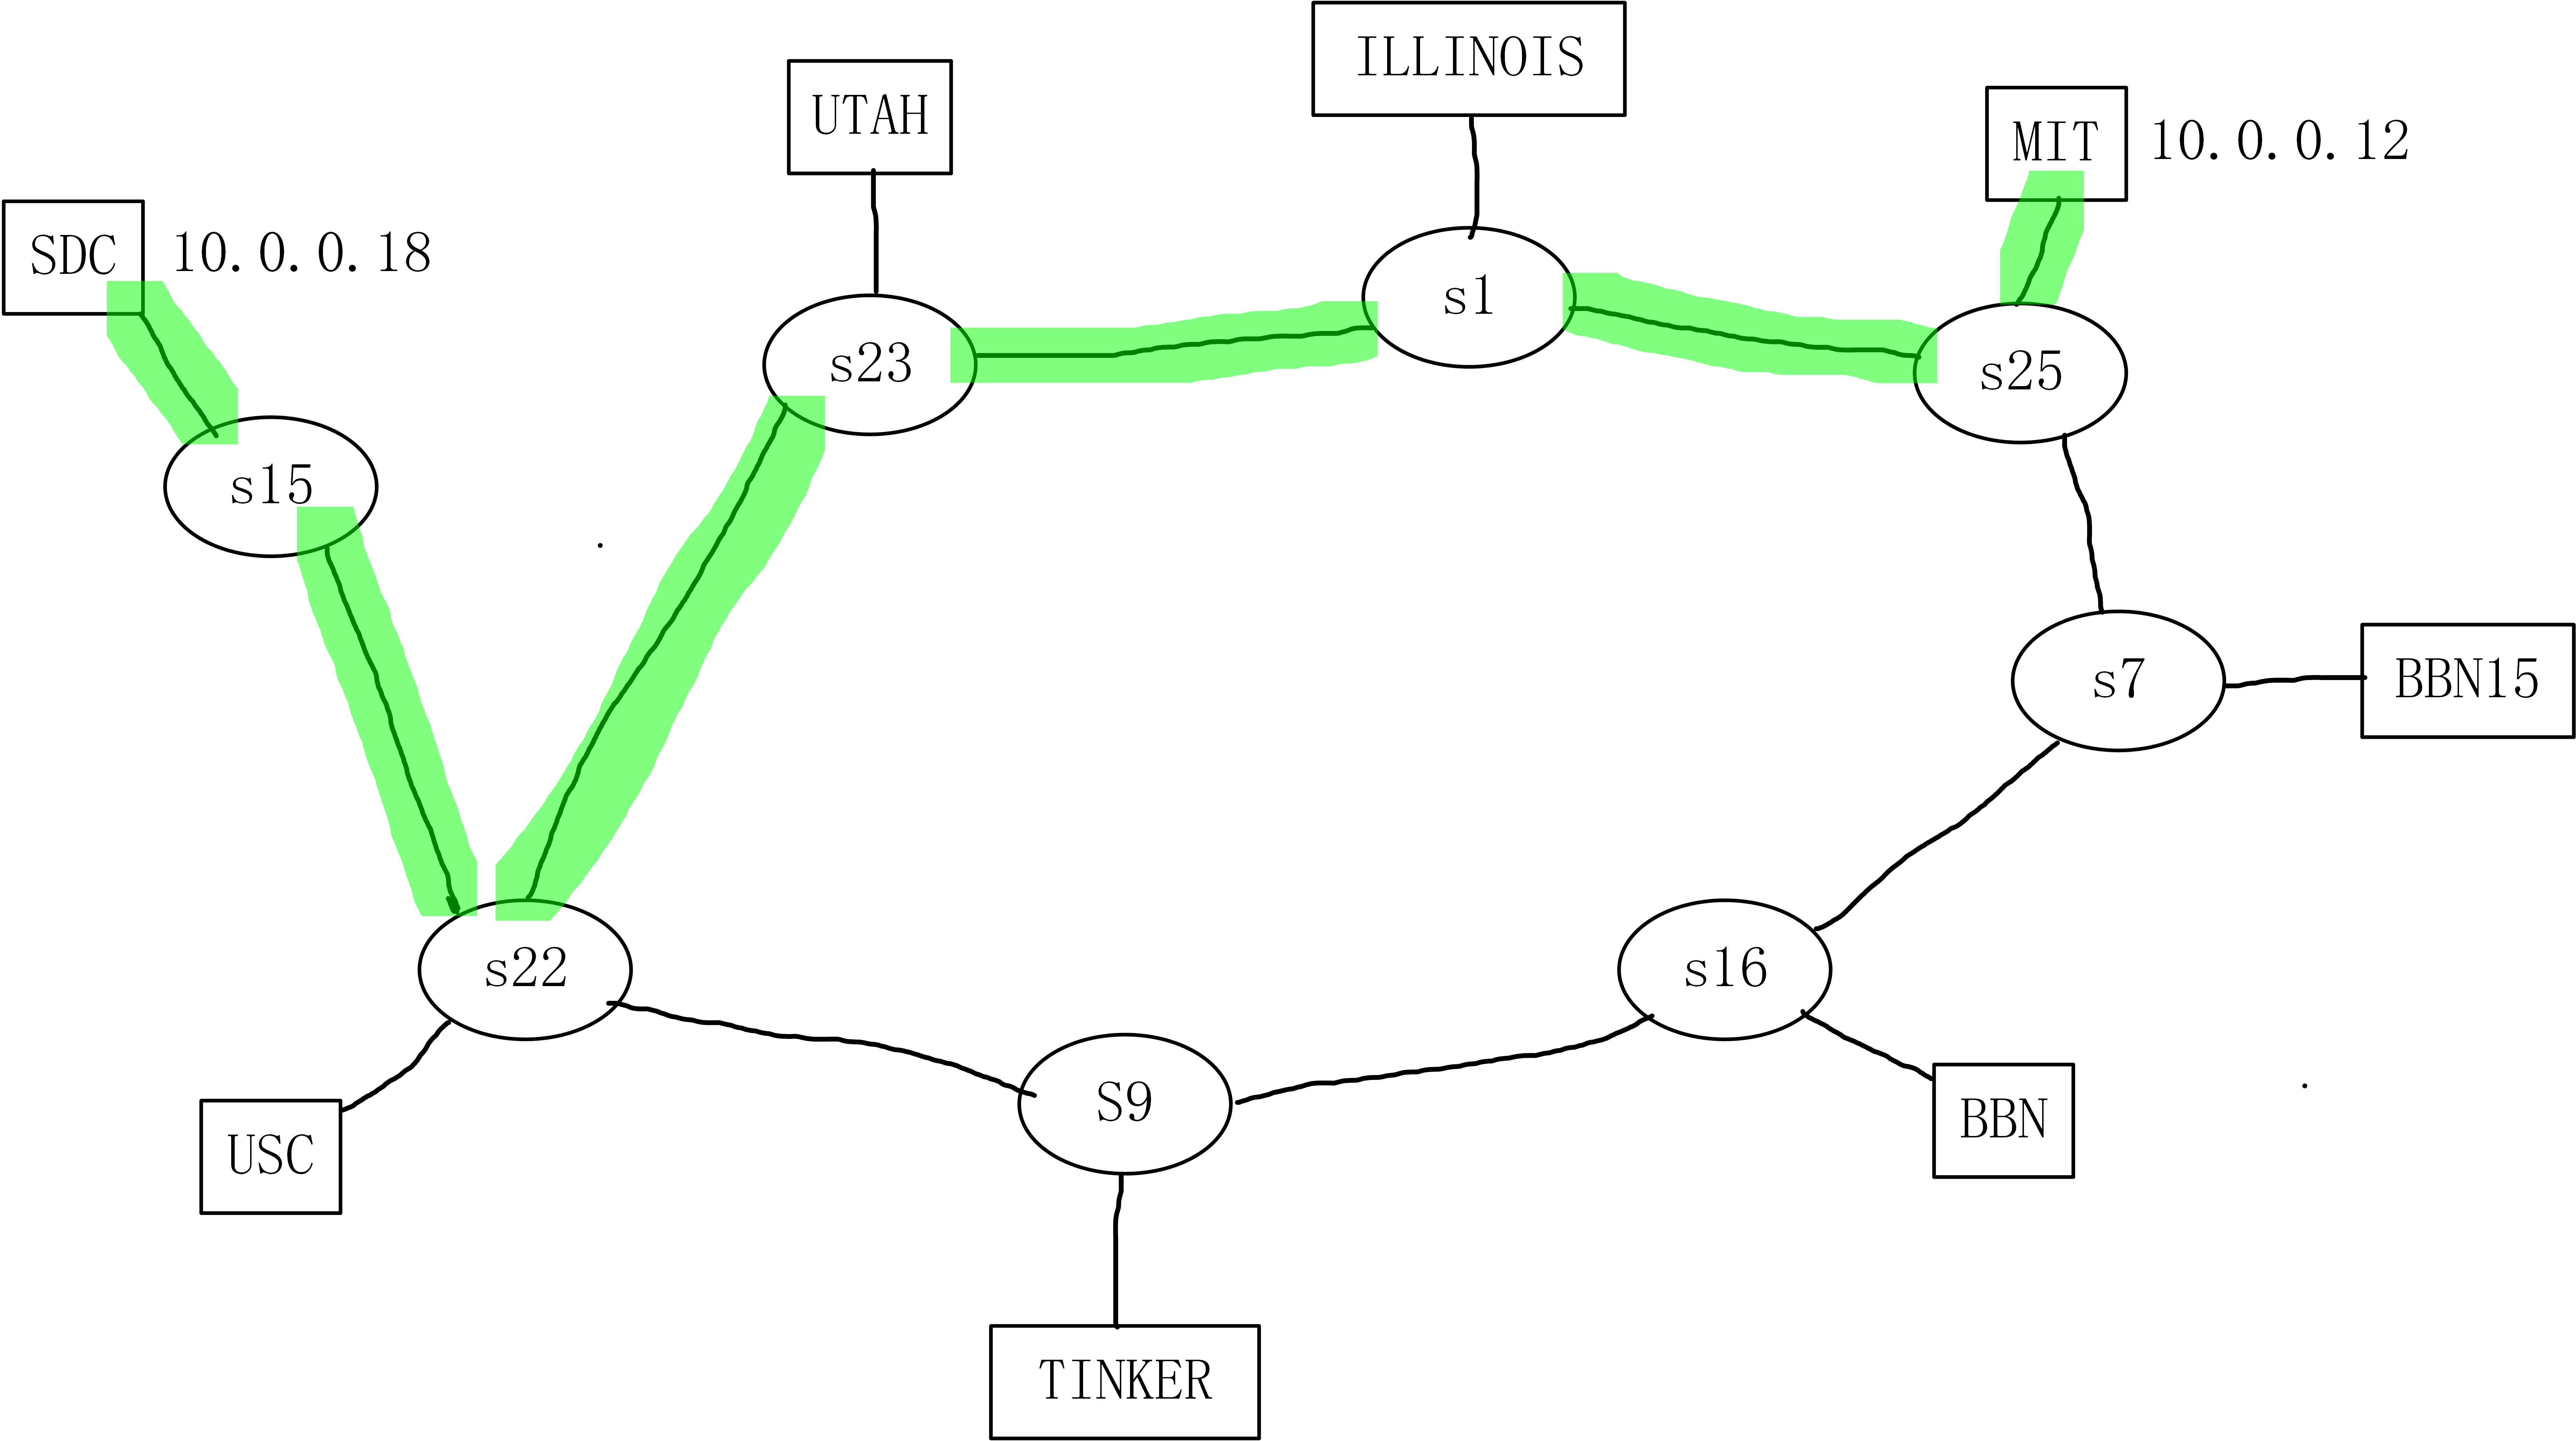
\includegraphics[width=0.8\linewidth]{4.jpg}
	\caption{UCSB Capture}
\end{figure}
\section{实验任务二:广播风暴}
\subsection{背景介绍}
\begin{figure}[H]
	\centering
	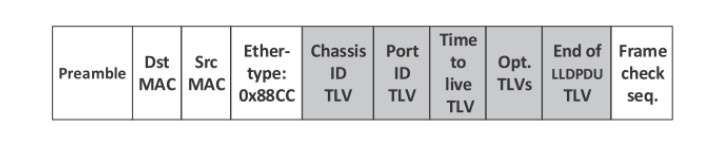
\includegraphics[width=0.8\linewidth]{2.jpg}
	\caption{ARPANET-2}
\end{figure}
\textbf{UCLA} 和 \textbf{UCSB} 通信频繁,两者间建立了一条直连链路。在新的拓扑 topo\_1969\_2.py 中运行自学习交换
机, \textbf{UCLA} 和 \textbf{UTAH} 之间无法正常通信。分析流表发现,源主机虽然只发了很少的几个数据包,但流表项
却匹配了上千次; WireShark 也截取到了数目异常大的相同报文\par 
\subsection{广播风暴及其解决思路}
这实际上是\textbf{ ARP }广播数据包在环状拓扑中洪泛导致的,传统网络利用\textbf{生成树协议}解决这一问题。在 \textbf{SDN}
中,不必局限于生成树协议,可以通过多种新的策略解决这一问题。以下给出一种解决思路,请在自学
习交换机的基础上完善代码,解决问题:\par
当序号为 \textbf{dpid} 的交换机从 \textbf{in\_port} 第一次收到某个 \textbf{src\_mac} 主机发出,询问 \textbf{dst\_ip} 的广播 \textbf{ARP Request} 数据包时,控制器记录一个映射 \textbf{(dpid, src\_mac, dst\_ip)->in\_port} 。下一次该交换机收到
同一 \textbf{(src\_mac, dst\_ip)} 但 \textbf{in\_port} 不同的 \textbf{ARP Request} 数据包时直接丢弃,否则洪泛。 
\subsection{关键代码设计思路}
在构造函数初始化一个表,维护一个(dpid,src\_mac,dst\_ip)->in\_port的映射。
\begin{lstlisting}[language=Python]
	self.sw = {}
\end{lstlisting}
\quad \quad 即对于arp包来说,问题在于如何分辨这个包是交换机转发而来还是主机发来的,既可以先存储一个表映射,arp包一定是主机先发起,所以先通过sw存储映射,表示只能从这个端口进入arp包,其他端口的arp包全部都要丢掉(因为其他端口的arp数据包是环路广播的结果),而对于其他交换机也是绑定端口和特定arp请求包的发送许可,从而实现广播风暴的避免,与生成树协议些许相似。对于符合映射的包正常转发,而不符合映射则丢弃,若没有对应映射,则进行学习,学习后正常转发。
\begin{lstlisting}[language=Python]	
if dst == ETHERNET_MULTICAST and ARP in header_list:
	arp_dst_ip = header_list[ARP].dst_ip
	if (dp.id, src, arp_dst_ip) in self.sw:
		if self.sw[(dp.id, src, arp_dst_ip)] != in_port:
			out = dp.ofproto_parser.OFPPacketOut(datapath=dp,
			buffer_id=dp.ofproto.OFP_NO_BUFFER,in_port=in_port,actions=[], data=None)
			dp.send_msg(out)
			return
		else:
			self.sw[(dp.id, src, arp_dst_ip)] = in_port
\end{lstlisting}
\subsection{运行结果与分析}
使用实验1的自学习交换机控制器来应用实验二,发现明显的广播风暴现象,流表匹配次数巨大。
\begin{figure}[H]
	\centering
	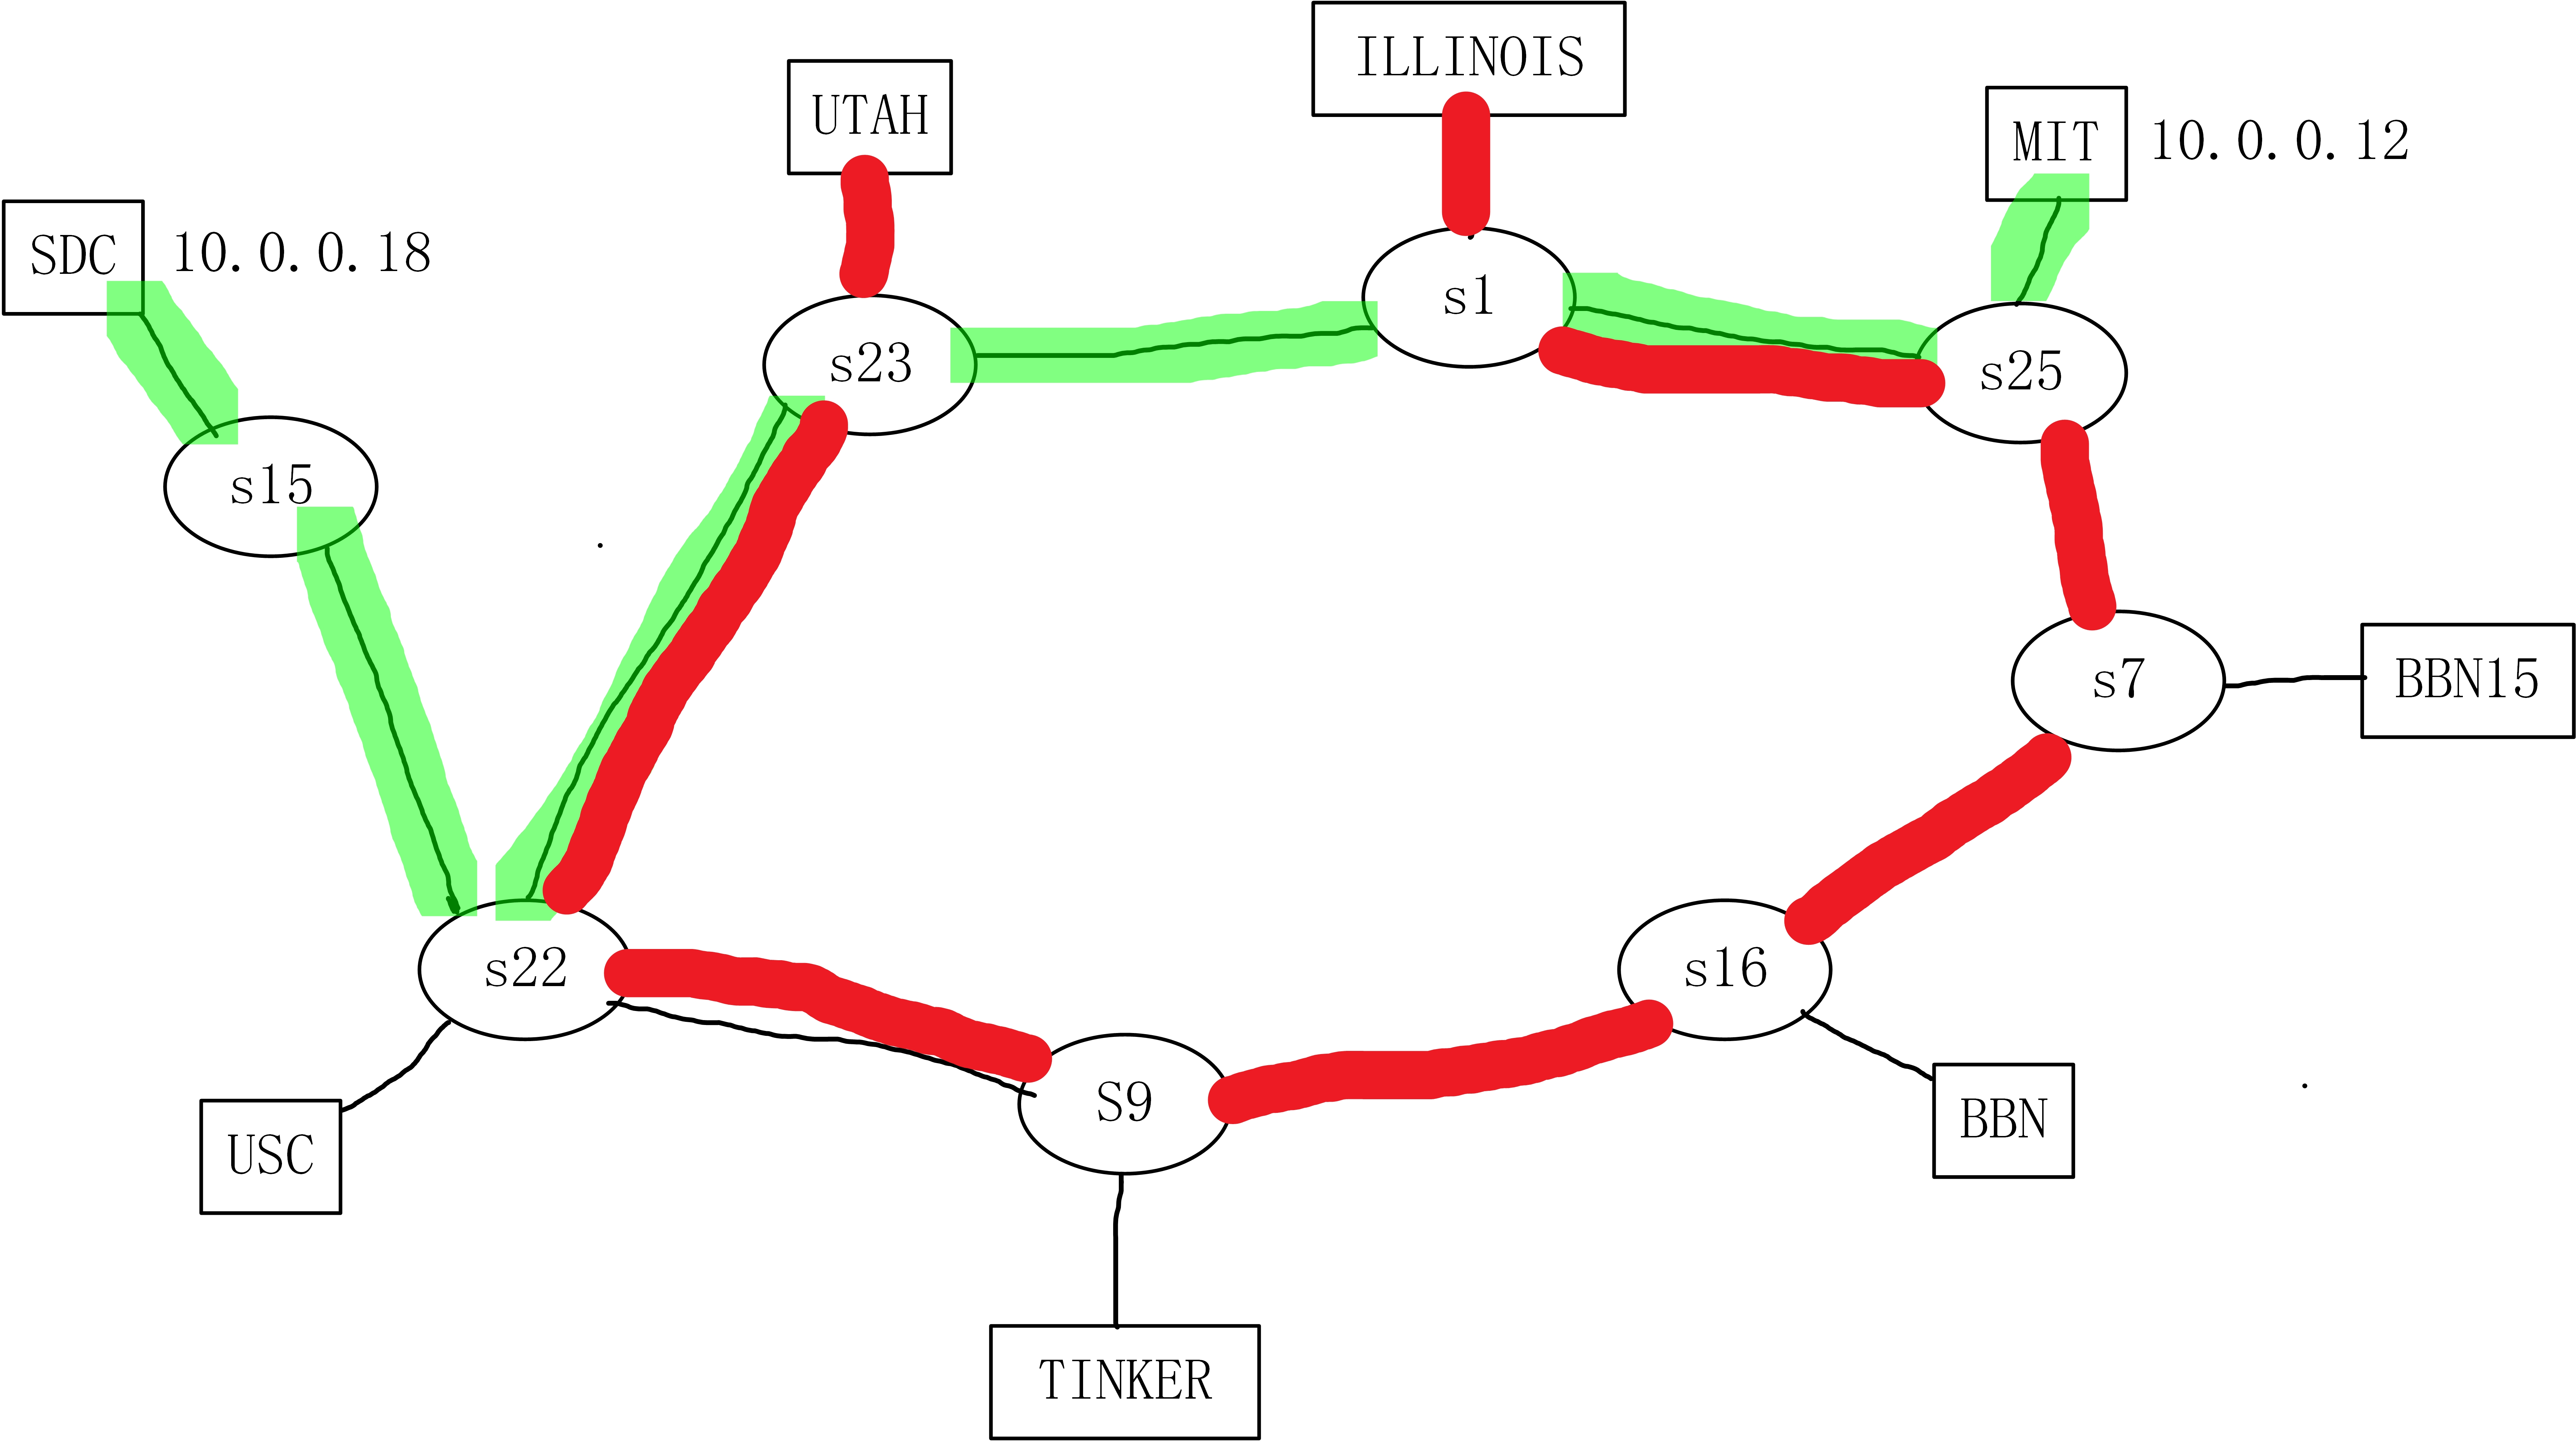
\includegraphics[width=1.0\linewidth]{6.jpg}
	\caption{解决前流表}
\end{figure}
\begin{figure}[H]
	\centering
	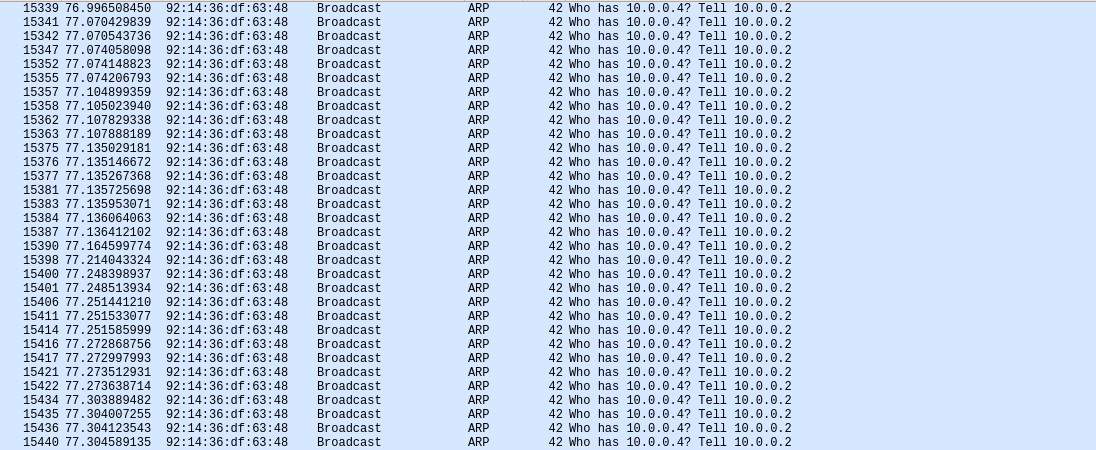
\includegraphics[width=1.0\linewidth]{7.jpg}
	\caption{解决前UCSB抓包}
\end{figure}
解决 ARP 数据包在环状拓扑中的洪泛问题后, UCLA 和 UTAH 之间可以 ping 通,并且流表项的匹配次数明显减少,UCSB监听也没有了广播风暴现象。
\begin{figure}[H]
	\centering
	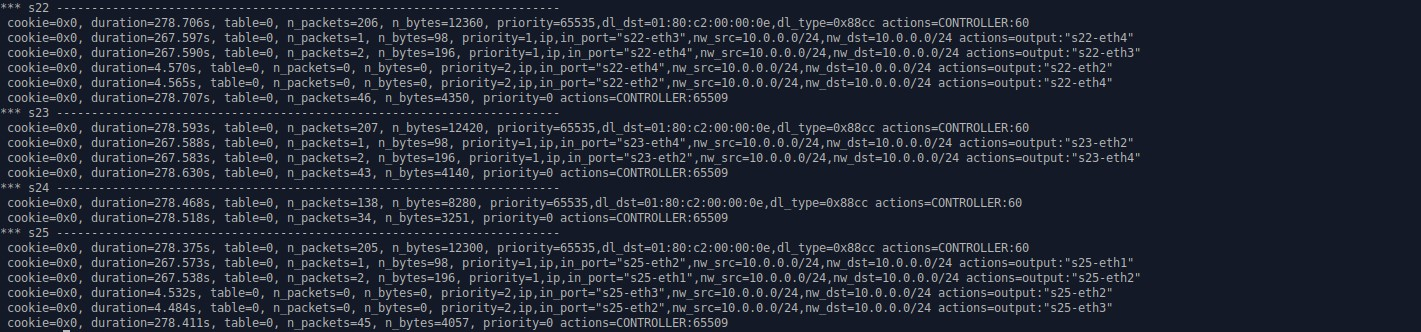
\includegraphics[width=1.0\linewidth]{5.jpg}
	\caption{解决后流表}
\end{figure}
\begin{figure}[H]
	\centering
	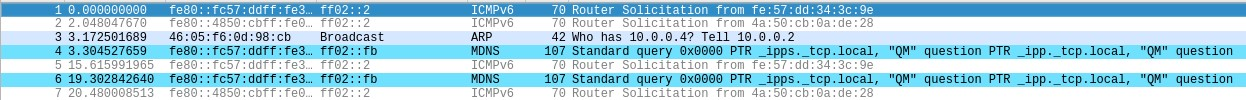
\includegraphics[width=1.0\linewidth]{8.jpg}
	\caption{解决后UCSB抓包}
\end{figure}
\subsection{方案优缺点分析}
优点:方法简单,实现成本低。\par 
缺点:实际上还是堵塞了某端口,占用了交换机链路带宽,每次需要丢包。\par
\section{实验任务三:附加方案}
\subsection{新的解决思路}
可以让控制器学习每个交换机与主机连接的mac地址和端口。直接让arp请求和响应报文不通过交换机链路,直接通过其他交换机交付主机。这样就不会出现arp广播风暴,示意图如图所示。
\begin{figure}[H]
	\centering
	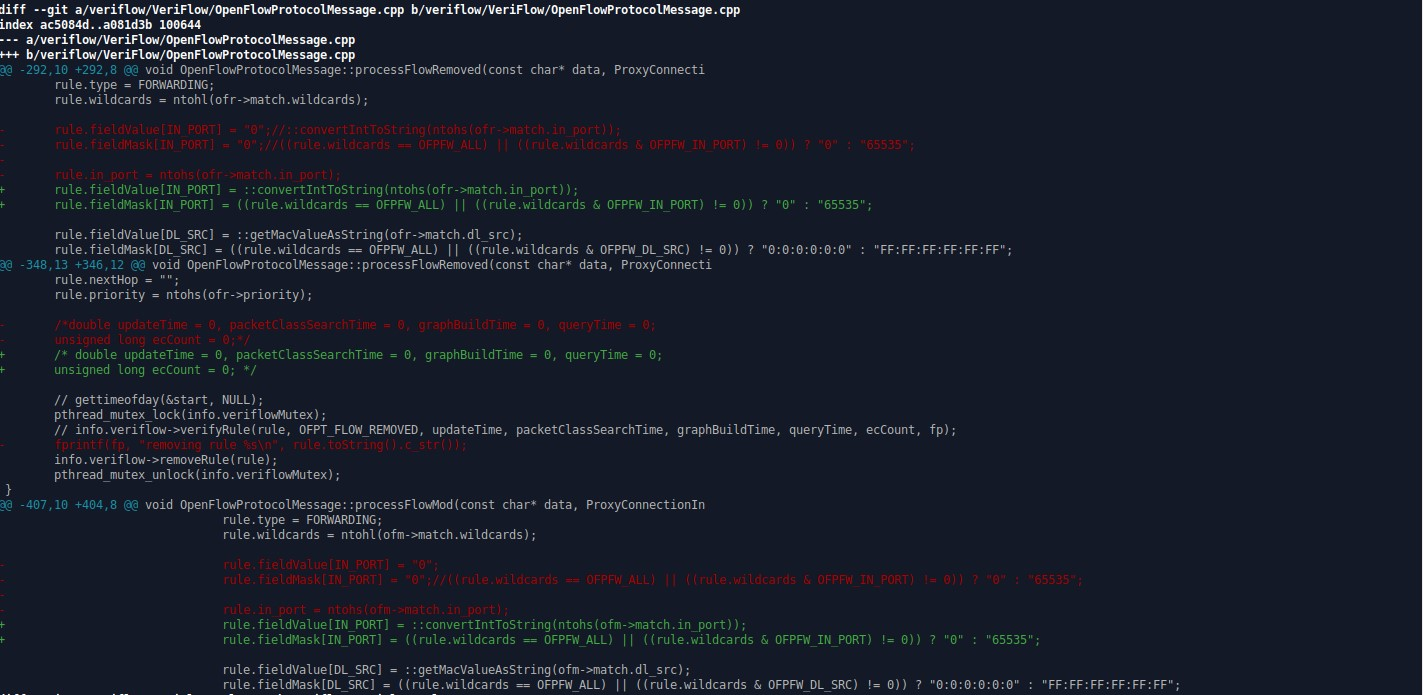
\includegraphics[width=0.8\linewidth]{9.jpg}
	\caption{解决后流表}
\end{figure}
\subsection{关键代码设计思路}
在构造函数初始化一个表,维护一个每个交换机主机和交换机端口的映射。
\begin{lstlisting}[language=Python]	
	self.host_mac_port = {}
\end{lstlisting}
\quad \quad 下面是一个实现上述机制的代码,首先分析是否为ARP包:\par
(1)如果是ARP包则查询src\_mac地址是否在该交换机的表中,如果在,则说明是正常发送,则其他交换机转发到连接的所有主机,如果不在,则说明不是正常发送,这时候学习src\_mac及其对应的交换机端口号,并且不处理arp 请求。
\begin{lstlisting}[language=Python]
if ARP in header_list:
	opcode = header_list[ARP].opcode
	if  opcode == arp.ARP_REQUEST:
		self.host_mac_port.setdefault(dp, {})
		if src in self.host_mac_port[dp]:
			for switch in self.host_mac_port.keys():
				ofp = switch.ofproto
				parser = switch.ofproto_parser
				for out_port in self.host_mac_port[switch].values():
					actions = [parser.OFPActionOutput(out_port)]
					out = parser.OFPPacketOut(datapath=switch,buffer_id=ofp.OFP_NO_BUFFER,
					in_port=ofp.OFPP_CONTROLLER,actions=actions, data=msg.data)
					switch.send_msg(out)
			return
		else:
			self.host_mac_port[dp][src] = in_port
			out = dp.ofproto_parser.OFPPacketOut(datapath=dp,buffer_id=dp.ofproto.OFP_NO_BUFFER
			,in_port=in_port,actions=[], data=None)
			dp.send_msg(out)
			return 
\end{lstlisting}
\quad \quad (2)如果是arp响应报文,则查询目的mac地址是否在表中,如果在某个交换机的表中,则某个交换机直接将arp响应报文发送给该主机,实现响应。
\begin{lstlisting}[language=Python]
	elif opcode == arp.ARP_REPLY:
		for switch in self.host_mac_port.keys():
			if dst in self.host_mac_port[switch]:
				ofp = switch.ofproto
				parser = switch.ofproto_parser
				out_port = self.host_mac_port[switch][dst]
				actions = [parser.OFPActionOutput(out_port)]
				out = parser.OFPPacketOut(datapath=switch,buffer_id=ofp.OFP_NO_BUFFER,
				in_port=ofp.OFPP_CONTROLLER,actions=actions, data=msg.data)
				switch.send_msg(out)
		return
\end{lstlisting}
\subsection{运行结果与分析}
解决 ARP 数据包在环状拓扑中的洪泛问题后, UCLA 和 UTAH 之间可以 ping 通,并且流表项的匹配次数明显减少,UCSB监听也没有了广播风暴现象。
\begin{figure}[H]
	\centering
	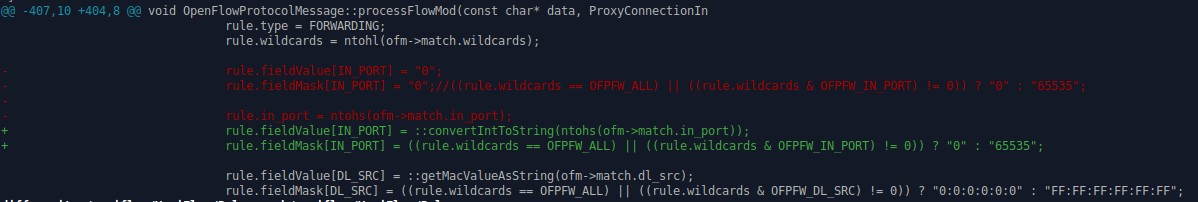
\includegraphics[width=0.9\linewidth]{10.jpg}
	\caption{流表匹配次数减少}
\end{figure}
所有节点能够成功ping通。
\begin{figure}[H]
	\centering
	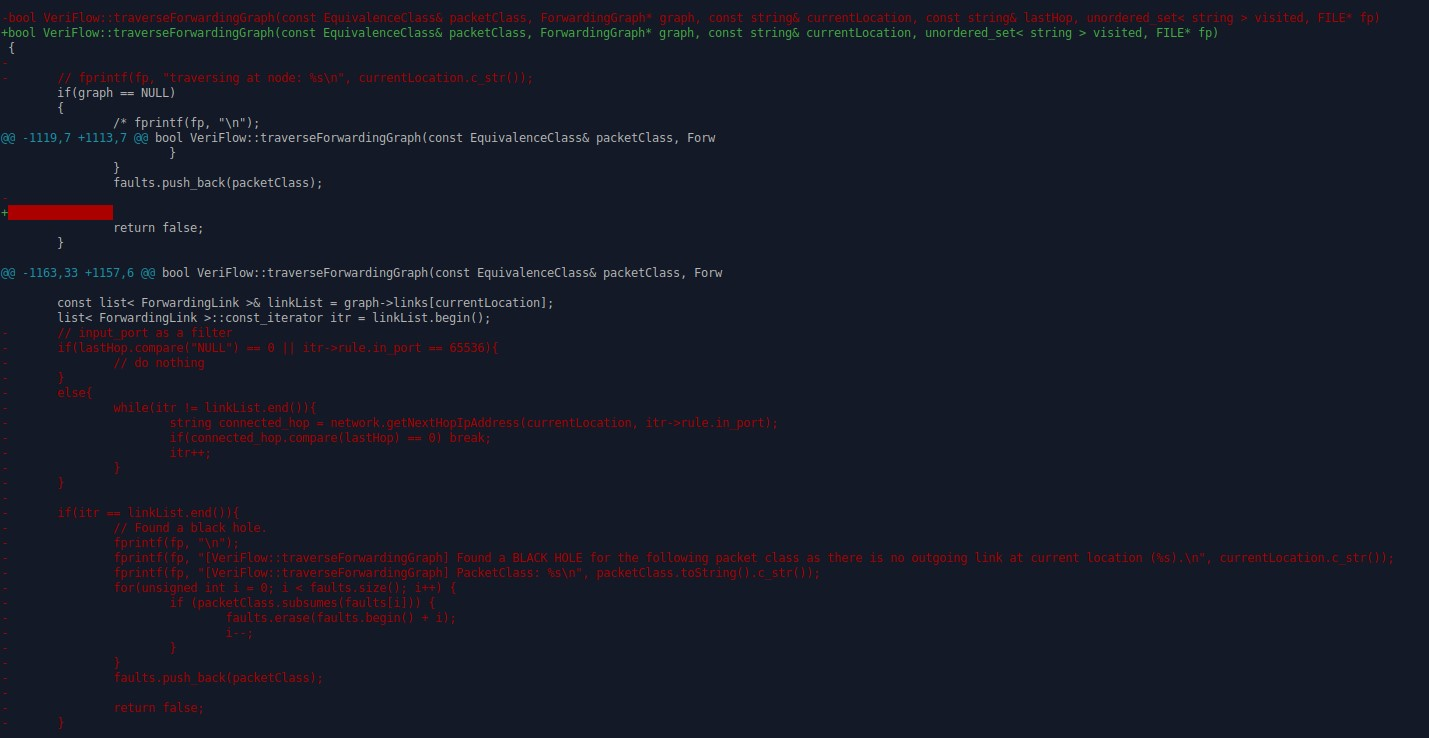
\includegraphics[width=0.9\linewidth]{11.jpg}
	\caption{能够成功ping通}
\end{figure}
在UTAH中抓包,发现能够正常抓包。
\begin{figure}[H]
	\centering
	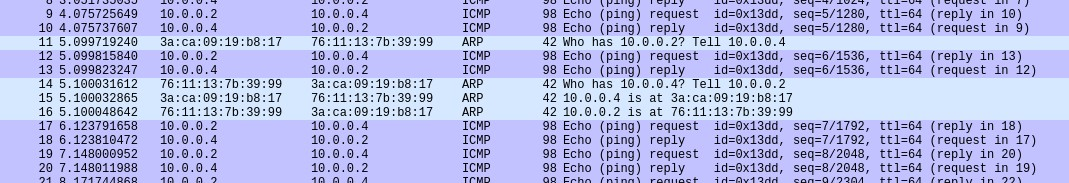
\includegraphics[width=0.9\linewidth]{12.jpg}
	\caption{UTAH抓包}
\end{figure}
可以在下图抓包发现,链路上并没有广播arp包,而是直接通过其他交换机广播发给主机,很好地实现了结果。
\begin{figure}[H]
	\centering
	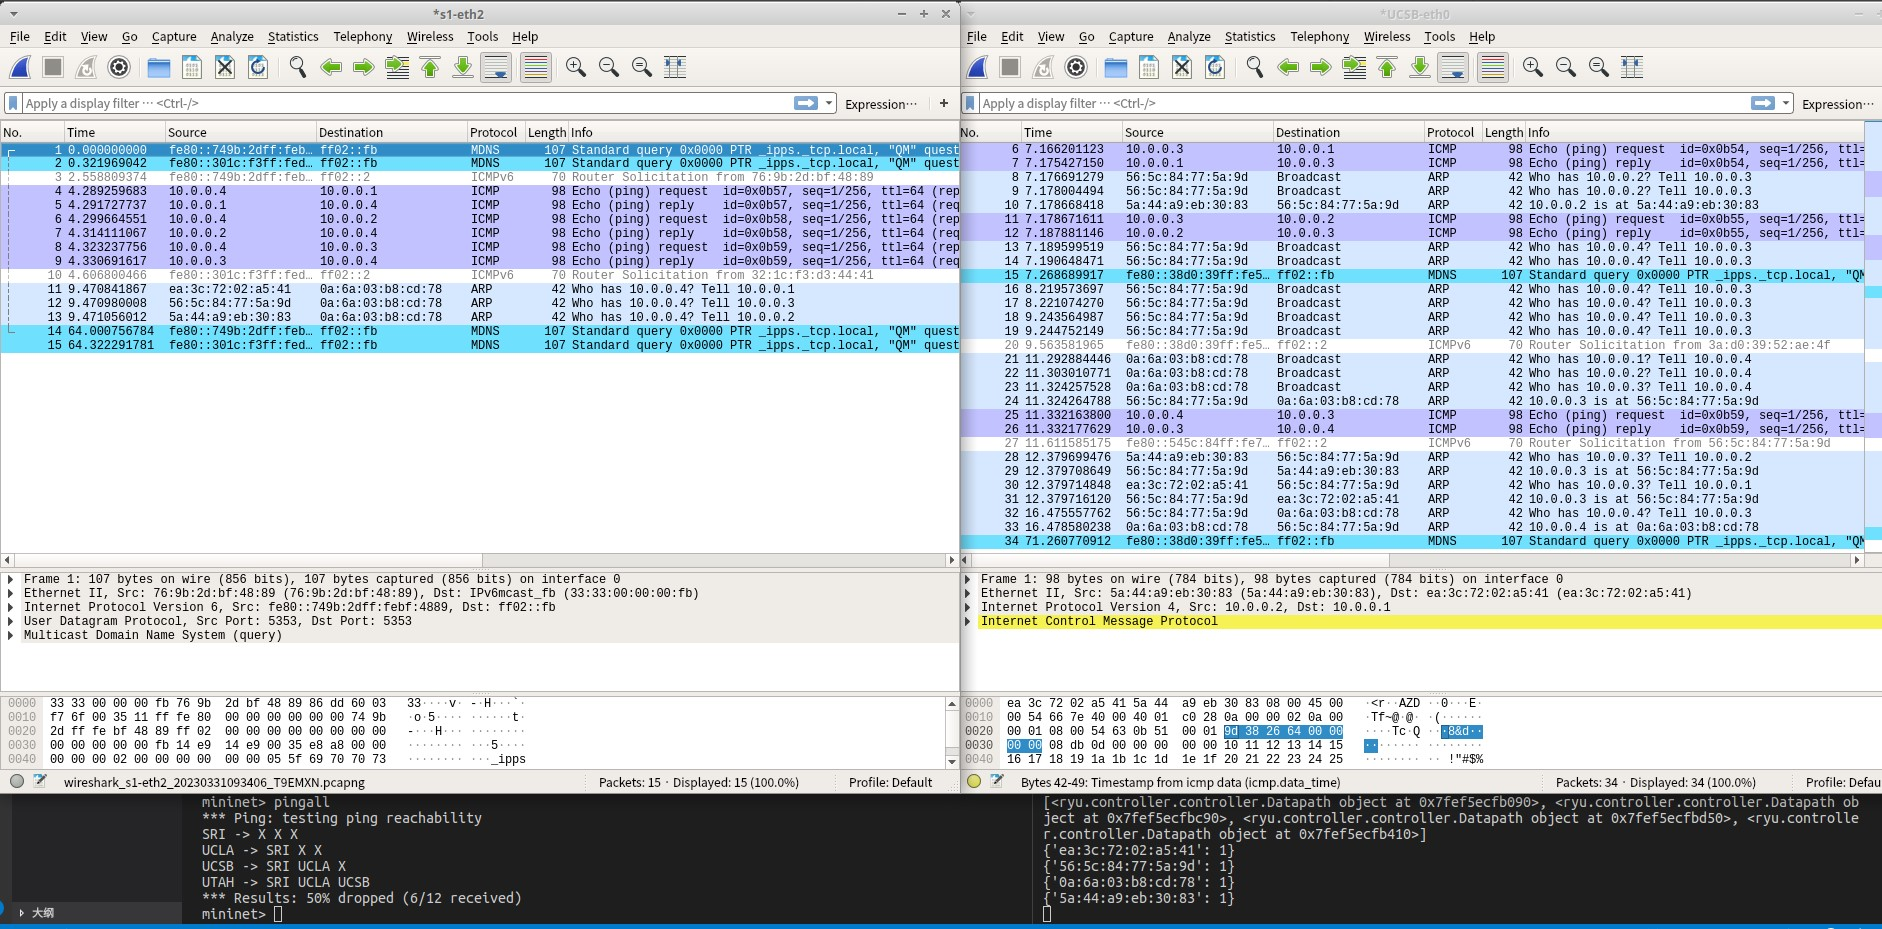
\includegraphics[width=1.0\linewidth]{13.jpg}
	\caption{交换机链路上并没有广播arp包}
\end{figure}
\subsection{方案优缺点分析}
优点:直接不占用交换机链路带宽,可以充分利用交换机的带宽。\par 
缺点:方法复杂,不够简洁,而且需要先ping来获取主机与端口绑定信息。没有办法对后期带有dst的arp请求报文进行处理,仍然会走交换机链路。\par
\section{附录}
\subsection{Learning\_Switch.py}
\begin{lstlisting}[language=Python]
from ryu.base import app_manager 
from ryu.controller import ofp_event 
from ryu.controller.handler import MAIN_DISPATCHER, CONFIG_DISPATCHER 
from ryu.controller.handler import set_ev_cls 
from ryu.ofproto import ofproto_v1_3 
from ryu.lib.packet import packet 
from ryu.lib.packet import ethernet 


class Switch(app_manager.RyuApp): 
	OFP_VERSIONS = [ofproto_v1_3.OFP_VERSION] 


	def __init__(self, *args, **kwargs): 
		super(Switch, self).__init__(*args, **kwargs)
		# maybe you need a global data structure to save the mapping 
		self.mac_to_port = {}

	def add_flow(self, datapath, priority, match, actions,idle_timeout=0,hard_timeout=0):
		dp = datapath 
		ofp = dp.ofproto 
		parser = dp.ofproto_parser 
		inst = [parser.OFPInstructionActions(ofp.OFPIT_APPLY_ACTIONS, actions)] 
		mod = parser.OFPFlowMod(datapath=dp, priority=priority, 
								idle_timeout=idle_timeout,
								hard_timeout=hard_timeout,
								match=match,instructions=inst) 
		dp.send_msg(mod) 

	@set_ev_cls(ofp_event.EventOFPSwitchFeatures, CONFIG_DISPATCHER) 
	def switch_features_handler(self, ev): 
		msg = ev.msg 
		dp = msg.datapath 
		ofp = dp.ofproto 
		parser = dp.ofproto_parser
		match = parser.OFPMatch() 
		actions = [parser.OFPActionOutput(ofp.OFPP_CONTROLLER,ofp.OFPCML_NO_BUFFER)] 
		self.add_flow(dp, 0, match, actions)

	@set_ev_cls(ofp_event.EventOFPPacketIn, MAIN_DISPATCHER) 
	def packet_in_handler(self, ev): 
		msg = ev.msg 
		dp = msg.datapath 
		ofp = dp.ofproto 
		parser = dp.ofproto_parser 

		# the identity of switch 
		dpid = dp.id 
		self.mac_to_port.setdefault(dpid,{}) 
		# the port that receive the packet 
		in_port = msg.match['in_port']
		pkt = packet.Packet(msg.data) 
		eth_pkt = pkt.get_protocol(ethernet.ethernet) 
		# get the mac 
		dst = eth_pkt.dst 
		src = eth_pkt.src 
		# we can use the logger to print some useful information 
		self.logger.info('packet: %s %s %s %s', dpid, src, dst, in_port)
		# you need to code here to avoid the direct flooding 
		# having fun 
		# :)
		# learn src mac -> port
		self.mac_to_port[dpid][src] = in_port
		#if match, then send to outport
		if dst in self.mac_to_port[dpid]:
			out_port = self.mac_to_port[dpid][dst]
		#if not match, then flood
		else:
			out_port = ofp.OFPP_FLOOD
		#pass information
		actions = [parser.OFPActionOutput(out_port)]
		
		if out_port != ofp.OFPP_FLOOD:
			match = parser.OFPMatch(in_port=in_port, eth_dst=dst, eth_src=src)
			self.add_flow(dp, 1, match, actions)
			
		data = msg.data
		out = parser.OFPPacketOut(datapath=dp,buffer_id=msg.buffer_id,in_port=in_port, actions=actions, data=data)
		dp.send_msg(out)
\end{lstlisting}
\subsection{Learning\_Switch\_Modified.py}
\begin{lstlisting}[language=Python]
from ryu.base import app_manager 
from ryu.controller import ofp_event 
from ryu.controller.handler import MAIN_DISPATCHER, CONFIG_DISPATCHER 
from ryu.controller.handler import set_ev_cls 
from ryu.ofproto import ofproto_v1_3 
from ryu.lib.packet import packet 
from ryu.lib.packet import ethernet 


class Switch(app_manager.RyuApp): 
	OFP_VERSIONS = [ofproto_v1_3.OFP_VERSION] 

	def __init__(self, *args, **kwargs): 
		super(Switch, self).__init__(*args, **kwargs)
		# maybe you need a global data structure to save the mapping 
		self.mac_to_port = {}

	def add_flow(self, datapath, priority, match, actions,buffer_id=None,idle_timeout=0,hard_timeout=0):
		dp = datapath 
		ofp = dp.ofproto 
		parser = dp.ofproto_parser 
		inst = [parser.OFPInstructionActions(ofp.OFPIT_APPLY_ACTIONS, actions)] 
		if buffer_id: 
			mod = parser.OFPFlowMod(datapath=datapath, priority=priority,buffer_id=buffer_id,idle_timeout=idle_timeout,
								hard_timeout=hard_timeout,match=match,instructions=inst)
		else:
			mod = parser.OFPFlowMod(datapath=datapath, priority=priority,idle_timeout=idle_timeout,
								hard_timeout=hard_timeout,match=match, instructions=inst)	
		dp.send_msg(mod) 

	@set_ev_cls(ofp_event.EventOFPSwitchFeatures, CONFIG_DISPATCHER) 
	def switch_features_handler(self, ev): 
		msg = ev.msg 
		dp = msg.datapath 
		ofp = dp.ofproto 
		parser = dp.ofproto_parser
		match = parser.OFPMatch() 
		actions = [parser.OFPActionOutput(ofp.OFPP_CONTROLLER,ofp.OFPCML_NO_BUFFER)] 
		self.add_flow(dp, 0, match, actions)

	@set_ev_cls(ofp_event.EventOFPPacketIn, MAIN_DISPATCHER) 
	def packet_in_handler(self, ev): 
		msg = ev.msg 
		dp = msg.datapath 
		ofp = dp.ofproto 
		parser = dp.ofproto_parser 

		# the identity of switch 
		dpid = dp.id 
		self.mac_to_port.setdefault(dpid,{}) 
		# the port that receive the packet 
		in_port = msg.match['in_port']
		pkt = packet.Packet(msg.data) 
		eth_pkt = pkt.get_protocol(ethernet.ethernet) 
		# get the mac 
		dst = eth_pkt.dst 
		src = eth_pkt.src 
		# we can use the logger to print some useful information 
		self.logger.info('packet: %s %s %s %s', dpid, src, dst, in_port)
		# you need to code here to avoid the direct flooding 
		# having fun 
		# :)
		# learn src mac -> port
		self.mac_to_port[dpid][src] = in_port
		#if match, then send to outport
		if dst in self.mac_to_port[dpid]:
			out_port = self.mac_to_port[dpid][dst]
		#if not match, then flood
		else:
			out_port = ofp.OFPP_FLOOD
		#pass information
		actions = [parser.OFPActionOutput(out_port)]

		if out_port != ofp.OFPP_FLOOD:
			match = parser.OFPMatch(in_port=in_port, eth_dst=dst, eth_src=src)
			if msg.buffer_id != ofp.OFP_NO_BUFFER:
				self.add_flow(dp, 1, match, actions, msg.buffer_id)
				return
			else:
				self.add_flow(dp, 1, match, actions)

		data = None
		if msg.buffer_id == ofp.OFP_NO_BUFFER:
			data = msg.data

		out = parser.OFPPacketOut(datapath=dp,buffer_id=msg.buffer_id,in_port=in_port, actions=actions, data=data)
		dp.send_msg(out)
\end{lstlisting}
\subsection{Broadcast\_Loop.py}
\begin{lstlisting}[language=Python]
from ryu.base import app_manager
from ryu.controller import ofp_event
from ryu.controller.handler import MAIN_DISPATCHER, CONFIG_DISPATCHER
from ryu.controller.handler import set_ev_cls
from ryu.ofproto import ofproto_v1_3
from ryu.lib.packet import packet
from ryu.lib.packet import ethernet
from ryu.lib.packet import arp
from ryu.lib.packet import ether_types

ETHERNET = ethernet.ethernet.__name__
ETHERNET_MULTICAST = "ff:ff:ff:ff:ff:ff"
ARP = arp.arp.__name__


class Switch_Dict(app_manager.RyuApp):
	OFP_VERSIONS = [ofproto_v1_3.OFP_VERSION]

	def __init__(self, *args, **kwargs):
		super(Switch_Dict, self).__init__(*args, **kwargs)
		self.sw = {} #(dpid, src_mac, dst_ip)=>in_port, you may use it in mission 2
		# maybe you need a global data structure to save the mapping
		# just data structure in mission 1
		self.mac_to_port = {}



	def add_flow(self, datapath, priority, match, actions, idle_timeout=0, hard_timeout=0):
		dp = datapath
		ofp = dp.ofproto
		parser = dp.ofproto_parser
		inst = [parser.OFPInstructionActions(ofp.OFPIT_APPLY_ACTIONS, actions)]
		mod = parser.OFPFlowMod(datapath=dp, priority=priority,
								idle_timeout=idle_timeout,
								hard_timeout=hard_timeout,
								match=match, instructions=inst)
		dp.send_msg(mod)

	@set_ev_cls(ofp_event.EventOFPSwitchFeatures, CONFIG_DISPATCHER)
	def switch_features_handler(self, ev):
		msg = ev.msg
		dp = msg.datapath
		ofp = dp.ofproto
		parser = dp.ofproto_parser
		match = parser.OFPMatch()
		actions = [parser.OFPActionOutput(ofp.OFPP_CONTROLLER, ofp.OFPCML_NO_BUFFER)]
		self.add_flow(dp, 0, match, actions)

	@set_ev_cls(ofp_event.EventOFPPacketIn, MAIN_DISPATCHER)
	def packet_in_handler(self, ev):
		msg = ev.msg
		dp = msg.datapath
		ofp = dp.ofproto
		parser = dp.ofproto_parser

		# the identity of switch
		dpid = dp.id
		self.mac_to_port.setdefault(dpid, {})
		# the port that receive the packet
		in_port = msg.match['in_port']
		pkt = packet.Packet(msg.data)
		eth_pkt = pkt.get_protocol(ethernet.ethernet)
		if eth_pkt.ethertype == ether_types.ETH_TYPE_LLDP:
			return
		if eth_pkt.ethertype == ether_types.ETH_TYPE_IPV6:
			return
		# get the mac
		dst = eth_pkt.dst
		src = eth_pkt.src
		# get protocols
		header_list = dict((p.protocol_name, p) for p in pkt.protocols if type(p) != str)
		if dst == ETHERNET_MULTICAST and ARP in header_list:
		# you need to code here to avoid broadcast loop to finish mission 2
			arp_dst_ip = header_list[ARP].dst_ip
			if (dp.id, src, arp_dst_ip) in self.sw:
				if self.sw[(dp.id, src, arp_dst_ip)] != in_port:
					out = dp.ofproto_parser.OFPPacketOut(datapath=dp,
					buffer_id=dp.ofproto.OFP_NO_BUFFER,
					in_port=in_port,actions=[], data=None)
					dp.send_msg(out)
					return
			else:
				self.sw[(dp.id, src, arp_dst_ip)] = in_port

		# self-learning
		# you need to code here to avoid the direct flooding 
		# having fun 
		# :)
		# just code in mission 1
		# learn src mac -> port
		self.mac_to_port[dpid][src] = in_port
		#if match, then send to outport
		if dst in self.mac_to_port[dpid]:
			out_port = self.mac_to_port[dpid][dst]
		#if not match, then fllink_list ood
		else:
			out_port = ofp.OFPP_FLOOD
		#pass information
		actions = [parser.OFPActionOutput(out_port)]

		if out_port != ofp.OFPP_FLOOD:
			match = parser.OFPMatch(in_port=in_port, eth_dst=dst, eth_src=src)
			self.add_flow(dp, 1, match, actions)

		data = None
		if msg.buffer_id == ofp.OFP_NO_BUFFER:
			data = msg.data

		out = parser.OFPPacketOut(datapath=dp,buffer_id=msg.buffer_id,in_port=in_port, actions=actions, data=data)
		dp.send_msg(out)
\end{lstlisting}
\subsection{Broadcast\_Loop2.py}
\begin{lstlisting}[language=Python]
from ryu.base import app_manager
from ryu.controller import ofp_event
from ryu.controller.handler import MAIN_DISPATCHER, CONFIG_DISPATCHER
from ryu.controller.handler import set_ev_cls
from ryu.ofproto import ofproto_v1_3
from ryu.lib.packet import packet
from ryu.lib.packet import ethernet
from ryu.lib.packet import arp
from ryu.lib.packet import ether_types


ETHERNET = ethernet.ethernet.__name__
ETHERNET_MULTICAST = "ff:ff:ff:ff:ff:ff"
ARP = arp.arp.__name__


class Switch_Dict(app_manager.RyuApp):
	OFP_VERSIONS = [ofproto_v1_3.OFP_VERSION]

	def __init__(self, *args, **kwargs):
		super(Switch_Dict, self).__init__(*args, **kwargs)
		self.mac_to_port = {}
		self.host_mac_port = {}


	def add_flow(self, datapath, priority, match, actions, idle_timeout=0, hard_timeout=0):
		dp = datapath
		ofp = dp.ofproto
		parser = dp.ofproto_parser
		inst = [parser.OFPInstructionActions(ofp.OFPIT_APPLY_ACTIONS, actions)]
		mod = parser.OFPFlowMod(datapath=dp, priority=priority,
								idle_timeout=idle_timeout,
								hard_timeout=hard_timeout,
								match=match, instructions=inst)
		dp.send_msg(mod)

	@set_ev_cls(ofp_event.EventOFPSwitchFeatures, CONFIG_DISPATCHER)
	def switch_features_handler(self, ev):
		msg = ev.msg
		dp = msg.datapath
		ofp = dp.ofproto
		parser = dp.ofproto_parser
		match = parser.OFPMatch()
		actions = [parser.OFPActionOutput(ofp.OFPP_CONTROLLER, ofp.OFPCML_NO_BUFFER)]
		self.add_flow(dp, 0, match, actions)

	@set_ev_cls(ofp_event.EventOFPPacketIn, MAIN_DISPATCHER)
	def packet_in_handler(self, ev):
		msg = ev.msg
		dp = msg.datapath
		ofp = dp.ofproto
		parser = dp.ofproto_parser


		# the identity of switch
		dpid = dp.id
		self.mac_to_port.setdefault(dp, {})
		# the port that receive the packet
		in_port = msg.match['in_port']
		pkt = packet.Packet(msg.data)
		eth_pkt = pkt.get_protocol(ethernet.ethernet)
		if eth_pkt.ethertype == ether_types.ETH_TYPE_LLDP:
			return
		if eth_pkt.ethertype == ether_types.ETH_TYPE_IPV6:
			return
		# get the mac
		dst = eth_pkt.dst
		src = eth_pkt.src

		# get protocols
		header_list = dict((p.protocol_name, p) for p in pkt.protocols if type(p) != str)

		self.mac_to_port[dp][src] = in_port
		if dst in self.mac_to_port[dp]:
			out_port = self.mac_to_port[dp][dst]
		else:
			out_port = ofp.OFPP_FLOOD
		actions = [parser.OFPActionOutput(out_port)]
		if out_port != ofp.OFPP_FLOOD:
			match = parser.OFPMatch(in_port=in_port, eth_dst=dst, eth_src=src)
			self.add_flow(dp, 1, match, actions)

		if ARP in header_list:
		# you need to code here to avoid broadcast loop to finish mission 2
			opcode = header_list[ARP].opcode
			if  opcode == arp.ARP_REQUEST:
				self.host_mac_port.setdefault(dp, {})
				if src in self.host_mac_port[dp]:
					for switch in self.host_mac_port.keys():
						ofp = switch.ofproto
						parser = switch.ofproto_parser
						for out_port in self.host_mac_port[switch].values():
							#print(out_port)
							actions = [parser.OFPActionOutput(out_port)]
							out = parser.OFPPacketOut(datapath=switch,buffer_id=ofp.OFP_NO_BUFFER,
							in_port=ofp.OFPP_CONTROLLER,actions=actions, data=msg.data)
							switch.send_msg(out)
					return
			else:
				self.host_mac_port[dp][src] = in_port
				return 

			elif opcode == arp.ARP_REPLY:
				for switch in self.host_mac_port.keys():
					if dst in self.host_mac_port[switch]:
						ofp = switch.ofproto
						parser = switch.ofproto_parser
						out_port = self.host_mac_port[switch][dst]
						actions = [parser.OFPActionOutput(out_port)]
						out = parser.OFPPacketOut(datapath=switch,buffer_id=ofp.OFP_NO_BUFFER,
						in_port=ofp.OFPP_CONTROLLER,actions=actions, data=msg.data)
						switch.send_msg(out)
				return

	data = None
	if msg.buffer_id == ofp.OFP_NO_BUFFER:
		data = msg.data
	out = parser.OFPPacketOut(datapath=dp,buffer_id=msg.buffer_id,in_port=in_port, actions=actions, data=data)
	dp.send_msg(out)	
\end{lstlisting}
\end{document}
